\section{Calculating frequentist limits} \label{S. Calculating limits}

Say that we have some test statistic $q$ which represents the compatibility between a model and the measurement of some observable. Larger values of $q$ mean that the observations become more and more likely under the model hypothesis. Say that we fix the model parameter $c_\text{model}$. Figure~\ref{F. CL from test-stat}(left) then shows a possible expected distribution of $q$. A single experiment is performed, and a value of $q_\text{obs}$ is measured. The \textbf{confidence level (CL)} of this observation is obtained by integrating the expected distribution (normalised to unity) between $-\infty$ and $q_\text{obs}$. This number represents the fraction of experiments which we would expect to produce a result less consistent with the model hypothesis than what was measured, if we assume that particular value of $c_\text{model}$.

\begin{figure}[t!]
\centering
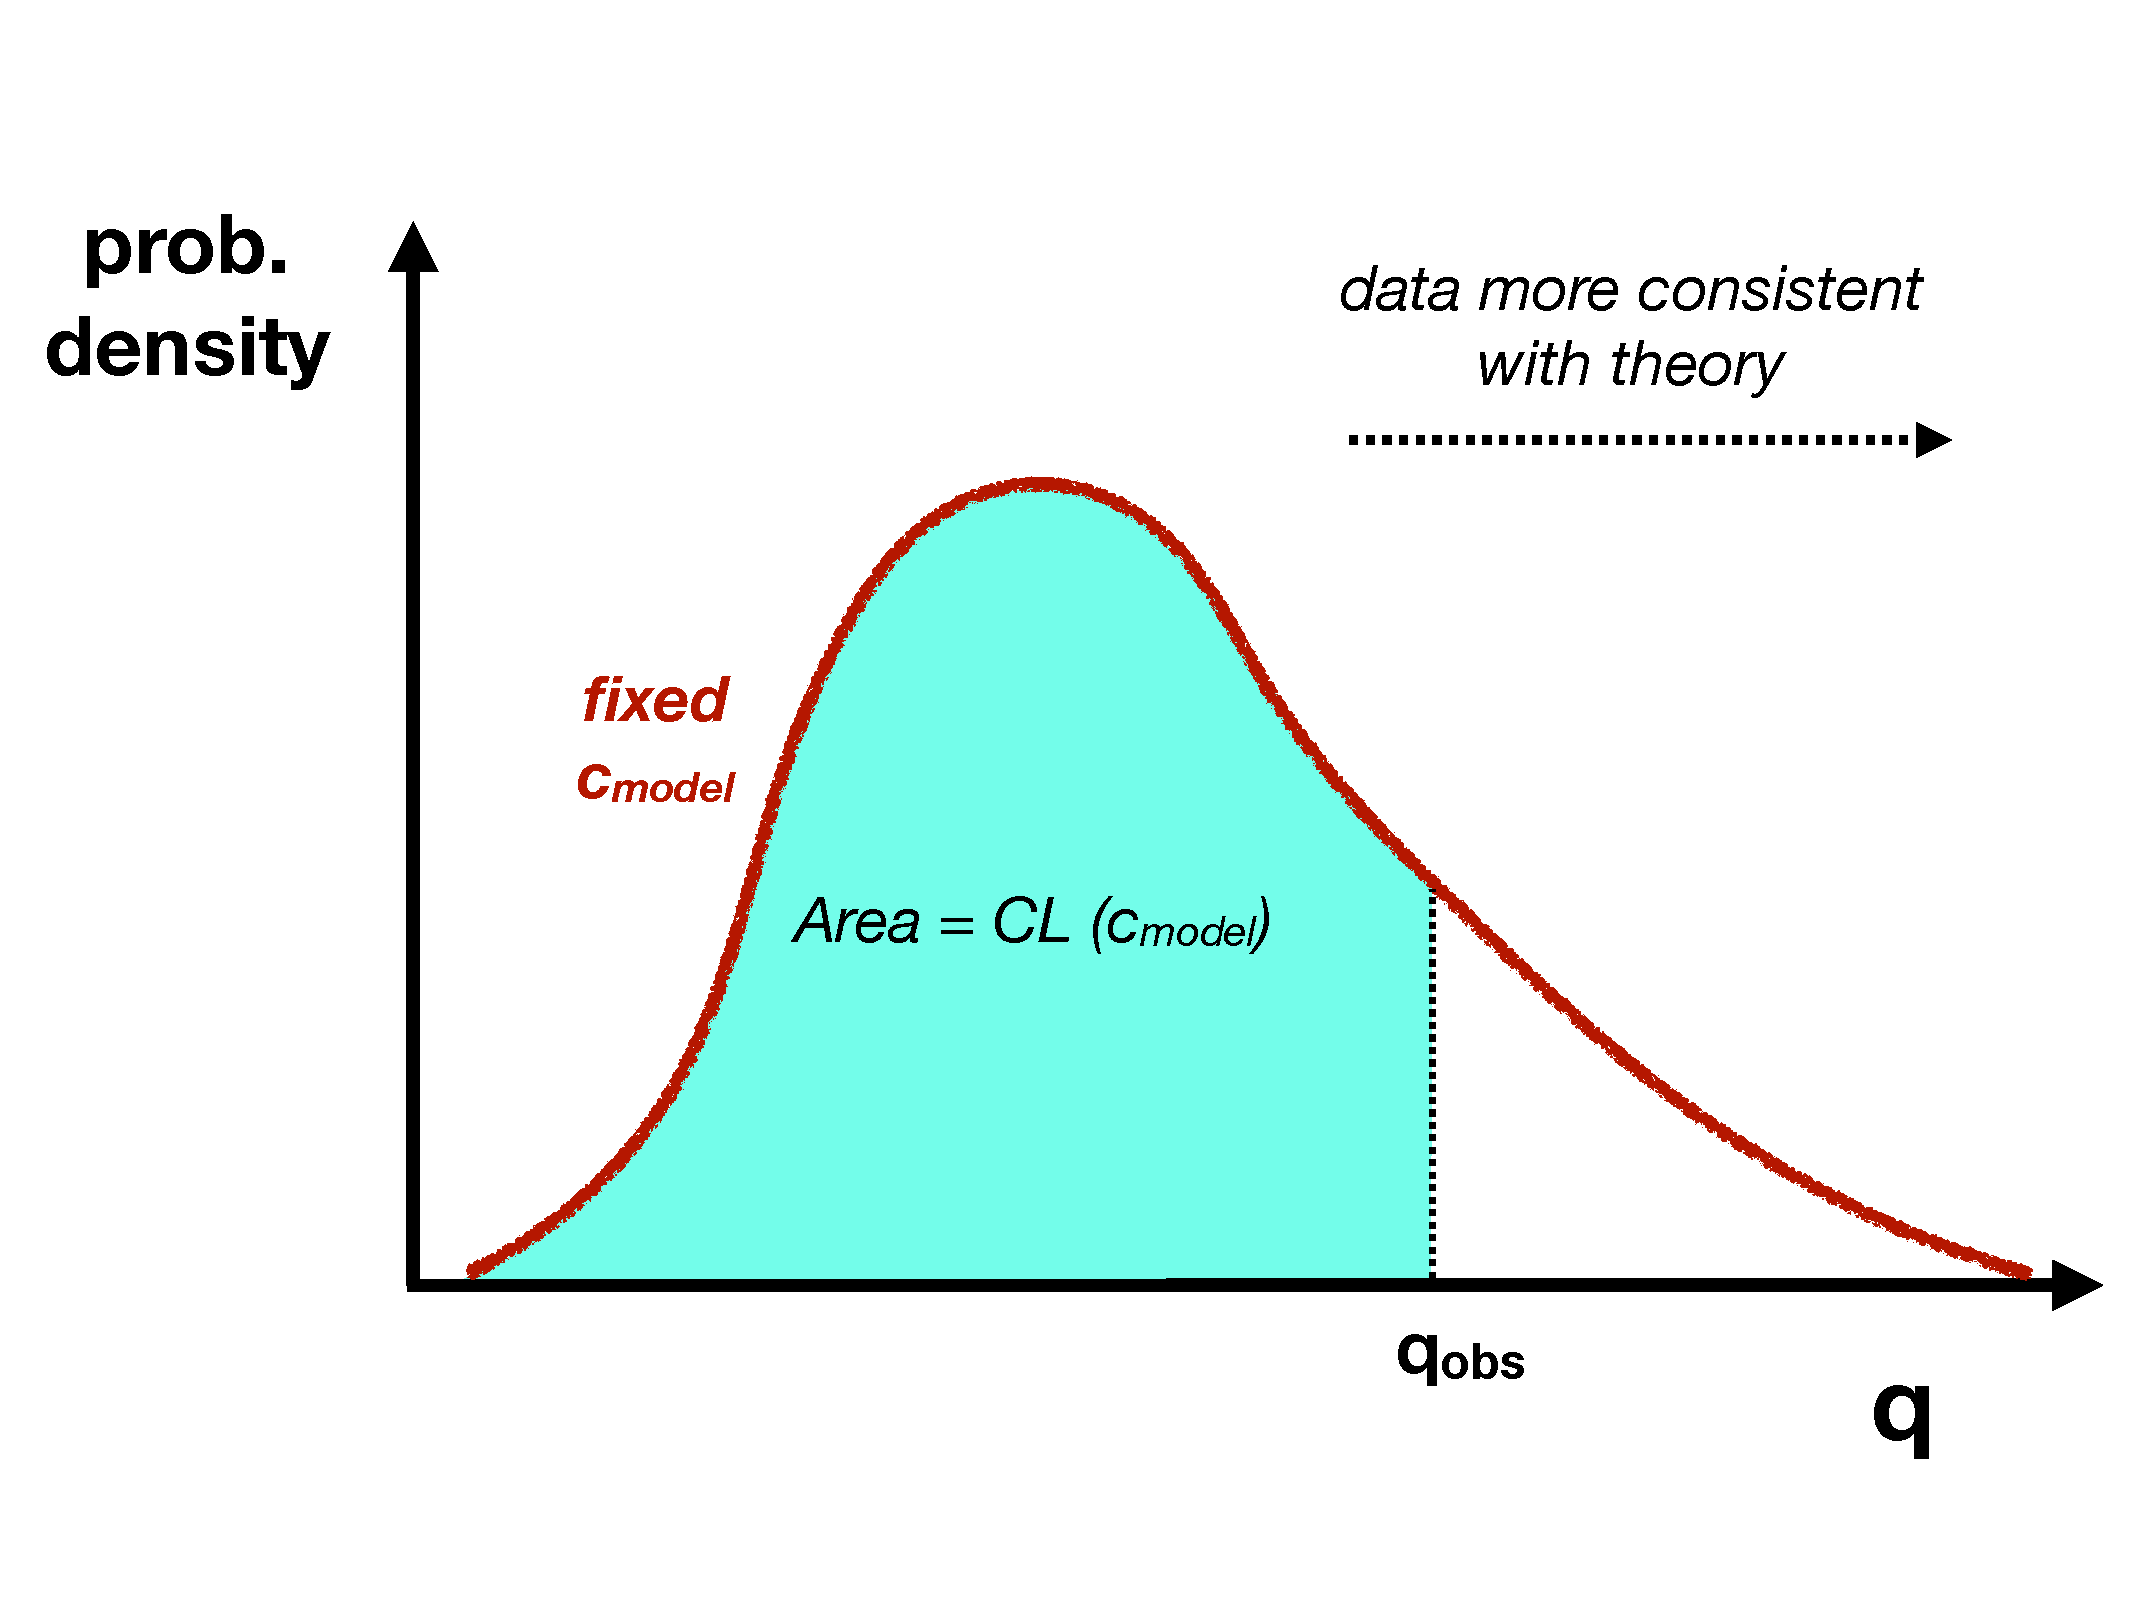
\includegraphics[page=1, width=0.49\textwidth]{TestStatisticDiagram.pdf}
\includegraphics[page=2, width=0.49\textwidth]{TestStatisticDiagram.pdf}
\caption{Left: diagram showing how $\textit{CL}\left(c_\text{model}\right)$ of a single experiment $q_\text{obs}$ is evaluated by integrating over the expected distribution of test statistic $q$ at each scan point in $c_\text{model}$. Right: diagram showing how a frequentist lower-limit on $c_\text{model}$ is extracted from the profile of  $\textit{CL}\left(c_\text{model}\right)$.}
\label{F. CL from test-stat}
\end{figure}

By scanning $c_\text{model}$, we obtain a profile of $\textit{CL}\left(c_\text{model}\right)$ for that experiment. The shape of this profile is dependent on the details of the test statistic measured and the model tested. An example is shown in Figure~\ref{F. CL from test-stat}(right). In this case a lower limit on $c_\text{model}$ is determined by evaluating the region for which $\textit{CL}<1-\alpha$.

\newpage
\noindent \textbf{Likelihood ratio as a test statistic}
\vspace{0.5cm}

The treatment up until now has been very general, not specific to any single model or test statistic. However, a common use-case in particle physics is the search for a signal where there exists an otherwise well-defined null hypothesis (the zero signal case). In this case a common test statistic is the \textbf{likelihood ratio}. The concept of a likelihood was introduced in the previous section. We re-iterate the definition here, now using the special notation $\mathcal{L}$ to denote this important quantity:

 \vspace{0.2cm}
 \begin{table}[h!]
 \begin{tabular}{lc}
\multirow{2}{*}{\textbf{\emph{Likelihood,}} $\mathcal{L}\left(\vec{x}|\vec{\theta}\right)$} \hspace{0.5cm}  & ``the probability density for obtaining a set of measurements  \\
&  $\vec{x}$ \textit{given} a model hypothesis and set of model parameters $\vec\theta$''
\end{tabular}
\end{table}

Note that the likelihood function is a PDF which is normalised over the domain of all possible \textit{measurements} $\vec{x}$, not all possible \textit{parameters} $\vec{\theta}$. This means that the likelihood should indeed be considered as a probabiltiy density, but not over the model parameters. This subtle difference becomes very important when interpreting likelihood profiles later on.

The vector $\vec{\theta}$ can contain so-called \textit{parameters of interest (PoIs)}, i.e. physical quantities which we want to measure or set limits on, and so-called \textit{nuisance parameters (NPs)}, i.e. further quantities which we do not know the true values of and wish to constrain using our data. Nuisance parameters are powerful tools which allow us to account for unknown quantities in our model, and especially for propagating the impact of systematic uncertainties onto the PoIs, however we will not consider this idea for now.

We can construct two models. The null hypothesis is described by a likelihood function of $\mathcal{L}_b\left(\vec{x}|\vec{\theta}_b\right)$. We can perform a \textit{maximum likelihood fit} which varies the NPs contained within $\vec{\theta}_b$ and finds the maximum likelihood $\mathcal{L}^\text{max}_b$. We say that the NPs have been \textit{marginalised}. A particular signal model is described by a likelihood $\mathcal{L}_{s+b}\left(\vec{x}|\vec{\theta}_{s+b}\right)$. In this case we find $\mathcal{L}^\text{max}_{s+b}$ by optimising all relevant PoIs and NPs. The likelihood ratio is defined as 
\begin{equation}
q =
\frac{ \mathcal{L}^\text{max}_{s+b}\left(\vec{x}|\vec{\theta}_{s+b}\right) }{ \mathcal{L}^\text{max}_b\left(\vec{x}|\vec{\theta}_b\right) } ~~~.
\end{equation}
This test statistic is designed to discriminate between measurements consistent with the ``signal plus background'' ($s+b$) and ``background only'' ($b$) hypotheses. It is large when the $s+b$ hypothesis had a significantly larger chance of producing the observed measurement than the $b$ hypothesis.

Note that we \textit{do not} fix $c_\text{model}$ within the fit of $\mathcal{L}^\text{max}_{s+b}\left(\vec{x}|\vec{\theta}_{s+b}\right)$ when evaluating $CL$ for a particular value of $c_\text{model}$. The fit is performed once for the $s+b$ hypothesis with $c_\text{model}$ floating (if even present), and once for the $b$ hypothesis, in order to determine $q_\text{obs}$. This single value is then used to evaluate $CL$ for many possible values of fixed $c_\text{model}$, for which the expected distributions of $q$ were derived in advance. We then evaluate limits using the prescription shown in Figure~\ref{F. CL from test-stat}. This is called the $\textit{CL}_{s+b}$ method. It is important to note that $CL_{s+b}$ results in true frequentist confidence intervals.

% Note that we can control model parameters such as $c_\text{model}$ within $\vec{\theta}_{s+b}$ and evaluate the confidence level at every scan point. 



